\chapter{Battle mechanics}
\label{chap:battle}
Pokémon GO features two major modes of battle: Nx1 and 3x3\footnote{These are commonly called PvE and PvP
 respectively. I don't like these terms, because Team GO Rocket encounters use the PvP format (despite involving
 a single Trainer), and Gyms use the PvE format (despite involving two Trainers).}.
Nx1 is used for raids, Max Battles, and (in a series of 1x1 matches) assaults on Gyms.
3x3 is used for encounters with Team GO Rocket and Trainer Battles.
All battles work on quanta of 0.5s\footnote{This is a recent change for Raid-style battling.}.
Aside from Trainer Battles, Trainers can make use of items in the screen before
  battle is entered (called the ``lobby'', especially in an Nx1 context), and
  likewise engage Mega evolutions.
Pokémon exchange fast attacks (and, when enough energy has been built up, charged attacks)
  until one side is entirely reduced to zero HP (or surrenders).

Remember that attacks typically have different power and energy stats depending on
  whether it's a 3x3 or Nx1 context (\autoref{chap:attacks}).
The fundamental ``damage equation'' is likewise calculated differently.
Each Attack reduces the opponent's Hit Points by some positive integer.
This integer is called (inflicted) damage $D$, and calculated as a product of several factors.

\section{The typing multiplier}
\label{sec:typemult}
Determine $M_C$, the common multiplier due typing:

\[ M_C = M_{STAB} \times 1.6^{T} \]

$M_{STAB}$ is the STAB bonus, equal to 1.2 when the Attack's Type matches any
  Type of the attacker, and 1 otherwise.
$T$ is the number calculated in \autoref{chap:types} using the Attack Type
 and the defender's Type.
I have included a $T$ of -4 in \autoref{table:typemult} for completeness,
 but remember that this is not currently realizable.

\begin{table}
\begin{center}
\begin{tabular}{c r r r r}
  $T$ & $1.6^{T}$ & Δ\% & w/ STAB & Δ\% \\
\Midrule
  -4 & 0.1526 & -84.74 & 0.1831 & -81.69 \\
  -3 & 0.2441 & -75.59 & 0.2930 & -70.7 \\
  -2 & 0.3906 & -60.94 & 0.4688 & -53.12 \\
  -1 & 0.625 & -37.5 & 0.75 & -25 \\
  0 & 1 & 0 & 1.2 & 20 \\
  1 & 1.6 & 60 & 1.92 & 92 \\
  2 & 2.56 & 156 & 3.072 & 207.2 \\
\end{tabular}
\caption{Typing multipliers with and without STAB}
\label{table:typemult}
\end{center}
\end{table}

Leaving out the hideous −4 case, we see that $M_C$ ranges
 from 0.2441 (a 75.59\% reduction in damage) to 3.072
 (a 207.2\% increase).
Considered another way, for an effectiveness of −3 with no STAB bonus,
 it takes about four times as many Attacks to subdue an opponent than
 we would otherwise expect.
With an effectiveness of 2 with STAB, it takes about one-third as many Attacks.

Note that the change due to a $T$ of 1 (60\%) is similar in magnitude to the change
 when $T$ is -2 (-60.94\%). A $T$ of -1 is a smaller loss (-37.5\%).
This does not mean that an Attack ineffective against one of the defender's types and
 effective against the other enjoys a 22.5\% gain (as one would see from $1.6^{-1} + 1.6^{1})$!
The multiplier is 1, and results in no change ($1.6^{-1+1}$).
The two effectiveness relationships must be added, and this value used to
 calculate $1.6^T$.
Exponential functions are not linear functions, and must not be treated as such.

\section{The context-specific multiplier}
\label{sec:mbmult}
In Raids and Max battles, a number of effects come into play.
\[ M_B = 0.5 \times M_D \times M_F \times M_W \times M_M \]
\begin{itemize}
 \item $M_D$ is 0.25 if the Attack is dodged (dodging is only possible in Raids/Max battles),
 and 1 otherwise. Note that this seems to have been subject to recent changes.
 \item The friendship bonus $M_F$:
   \begin{table}[h!]
\centering
       \begin{tabular}{lc}
         Situation & $M_F$ \\
         \Midrule
         No friends present, \textit{unless…} & 1 \\
         Battling with at least one Good Friend, \textit{unless…} & 1.03 \\
         Battling with at least one Great Friend, \textit{unless…}  & 1.05 \\
         Battling with at least one Ultra Friend, \textit{unless…} & 1.07 \\
         Battling with at least one Best Friend. & 1.1
       \end{tabular}
     \caption{Bonus due the presence of friends}
   \end{table}
 \item $M_W$ is 1.2 if the Attack is weather-boosted, and 1 otherwise.
 \item $M_M$ from Mega Pokémon \textit{actively} involved in a Raid (i.e. they
   must be fighting, not just on the team), or Primal Pokémon \textit{present}
   (even knocked out) at a Raid or Gym. The Primal bonus is not awarded to the Trainer who brought
   that Primal Pokémon, but they can receive it from some other Trainer's Pokémon.
   \begin{table}[h!]
     \centering
       \begin{tabular}{p{.7\textwidth}c}
         Situation & $M_M$ \\
         \Midrule
         No active Mega Pokémon, and no Primal Pokémon brought
          by other Trainers present, \textit{unless…} & 1 \\
         Battling with at least one Mega Pokémon,
          or another Trainer's Primal Pokémon present, \textit{unless…} & 1.1 \\
         Battling with at least one Mega Pokémon of the attack's type,
          or another Trainer's Primal Pokémon is present and of
          the attack's type. & 1.3 \\
       \end{tabular}
     \caption{Bonus due the presence of Mega and Primal Pokémon}
   \end{table}
   In a Max battle, $M_M$ is based on the number of Pokémon left at that Power Stop
     (see \autoref{sec:maxbattles}).
   \begin{table}[h!]
     \centering
       \begin{tabular}{lc}
         Pokémon present at Power Stop & $M_M$ \\
         \Midrule
         0 & 1 \\
         1 & 1.1 \\
         2--3 & 1.15 \\
         4--14 & 1.188 \\
         15+ & 1.2 \\
       \end{tabular}
     \caption{Bonus in Max battles due Pokémon at Power Stop}
   \end{table}
\end{itemize}
The calculation for Trainer Battles is simpler:
\[ M_B = 0.65 \times M_G \]
For Fast Attacks, $M_G$ is 1.
When throwing a Charged Attack, the attacking Trainer plays a short minigame.
Performance on this minigame is summarized with ``Excellent!'', ``Great!'',
``Nice!'', or silence.
This summary is a low-resolution signal of $M_G$, with a range over [0.25, 1].
``Excellent!'' is necessary and sufficient for a 1, and should always be obtainable.
\begin{table}
\centering
\begin{tabular}{l r}
Summary & $M_G$ range (no Shield) \\
\Midrule
``Excellent!'' & 1 \\
``Great!'' & [0.75, 1) \\
``Nice!'' & [0.5, 0.75) \\
No summary & [0.25, 0.5) \\
\end{tabular}
\caption{The minigame summary is an indication of $M_G$}
\end{table}
Each Trainer gets two shields in a battle, each of which can be used
 to block a single Charged Attack.
If a shield is used, $M_G$ is 0, no matter the minigame performance.
The effect is equivalent to raising the defender's DEF to infinity for the
  duration of the Attack.

\section{The damage equation}
\label{sec:damage}

$D_A$ is what we can calculate using only the attacker's knowledge, i.e.
 it is that component of $D$ which is independent of the defender.

\[ D_A = P \times Eff_A \times M_{STAB} \times M_B \]

Since this is a product, a proportional increase in any factor leads to
 the same change.
Suppose a Level 12 Pokémon (CPM: 0.4628) with $Mod_A$ of 140 runs
  a Fast Attack with a Power of 10 and no STAB bonus.
The resulting $D_A$ is 421.148.
Increasing Power to 12,
 increasing $Mod_A$ to 168,
 acquiring the STAB bonus,
 or increasing CPM 20\% to 0.55536 (somewhere between Levels 17 and 17.5; this exact change is not possible)
 all yield a 20\% increase in $D_A$, 505.3776.
Note that this is all independent of the opponent.

$D_A$ is divided by $Eff_D$ and scaled by $1.6^T$:

\[ D_D = \frac{D_A}{Eff_D} \times 1.6^T \]

We can recover our defined multipliers:

\[ D_D = P \times \frac{Eff_A}{Eff_D} \times M_C \times M_B \]

Using the definitions of $Eff_A$ and $Eff_D$, this can be rewritten as:

\[ D_D = P \times \frac{Mod_A \times CPM_A}{Mod_D \times CPM_D} \times M_C \times M_B \]

which can of course be rewritten as:

\[ D_D = P \times \frac{Mod_A}{Mod_D} \times \frac{CPM_A}{CPM_D} \times M_C \times M_B \]

A floor function is applied to ensure an integer,
 followed by a min function to ensure at least 1 point of damage is always inflicted:

\[ D = \min{1, \left\lfloor P \times \frac{Eff_A}{Eff_D} \times M_C \times M_B \right\rfloor } \]

If $D$ equals or exceeds the opponent's HP, it will fight no more.

\section{Opponent-independent damage}
We can break the damage equation into those parts dependent
 upon opponents, and those which are independent.
Looking at the damage equation, Power, $Eff_A$, and STAB do not depend
 upon an attacker's opponent.
Likewise $Eff_D$ and MHP for the defender.
The attacker knows neither $Eff_D$ nor MHP, while the defender doesn't know $Eff_A$.
Knowing type effectiveness always requires knowing the opposing typing.
We can thus define an independent core fitness evaluation:

\[ F = Eff_A \times P \times M_{STAB} \times Eff_D \times MHP \]

Note that CPM is implicitly cubed in this function.

Of course, a given Pokémon can generally select from multiple Fast and Charged Attacks,
  knowing up to two of the latter at a given time.
Furthermore, Fast and Charged Attacks are not used in equal ratio (there will
  always be multiple Fast Attacks per Charged Attack), and a Shield can
  nullify a Charged Attack.
How do we define $P$ and $M_{STAB}$?
As only one Fast Attack can be known at a time, it's easy enough to define one
  fitness for each possible Fast Attack, leaving out Charged Attacks for now.
All we need do is normalize the Power of the Fast Attack, using the number of
  Turns it requires.

\[ F = Eff_A \times \frac{P_{Fast}}{T_{Fast}} \times M_{STAB-Fast} \times Eff_D \times Eff_S \]

Integrating Charged Attacks is more complex.
First, we can simply normalize the Charged Attack as we did the Fast Attack,
 determine the number of Fast Attacks necessary to launch it:

\[ N_{Fast} = \lceil\frac{E_{Charged}}{E_{Fast}}\rceil \]

yielding the total Power of a cycle.

\[ TDO = N_{Fast} \times P_{Fast} + P_{Charged} \]

We normalize this by the turns of a full cycle:

\[ F_{cycle} = \frac{TDO}{N_{Fast} \times T_{Fast} + T_{Charged}} \]

There are two turns per second. Multiplying $F_{cycle}$ by two yields a
  stat the community calls Damage Per Second (DPS).

This has several problems, almost all related to Charged Attacks.
It doesn't account for the possibility of knowing two Charged Attacks.
It doesn't account for leftover Energy, which will sometimes be present if
  $E_{Charged}$ is not a multiple of $E_{Fast}$ (i.e. $N_{Fast}$
  might fluctuate from one cycle to the next).
It ignores the possibility that the attacker might not use its Charged Attack
  immediately (and it is often unwise to throw Charged Attacks as quickly as
  possible; see \autoref{chap:strategy}).
Finally, it presumes that the attacker can always get off a full cycle.
In reality, the attacker might be knocked out or substituted long before its
  Charged Attack becomes relevant, or the defender might use a Shield.
It is tempting to ignore Charged Attacks, but when they land, they tend to
  dominate our total inflicted damage\footnote{When a Charged Attack is thrown
  early against a lengthy fast attack, it allows for a ``free fast attack''
  (see \autoref{chap:battle}). This needn't be taken into account, as it is
  technically imperfect play.}.

\begin{figure}[ht]
  \centering
  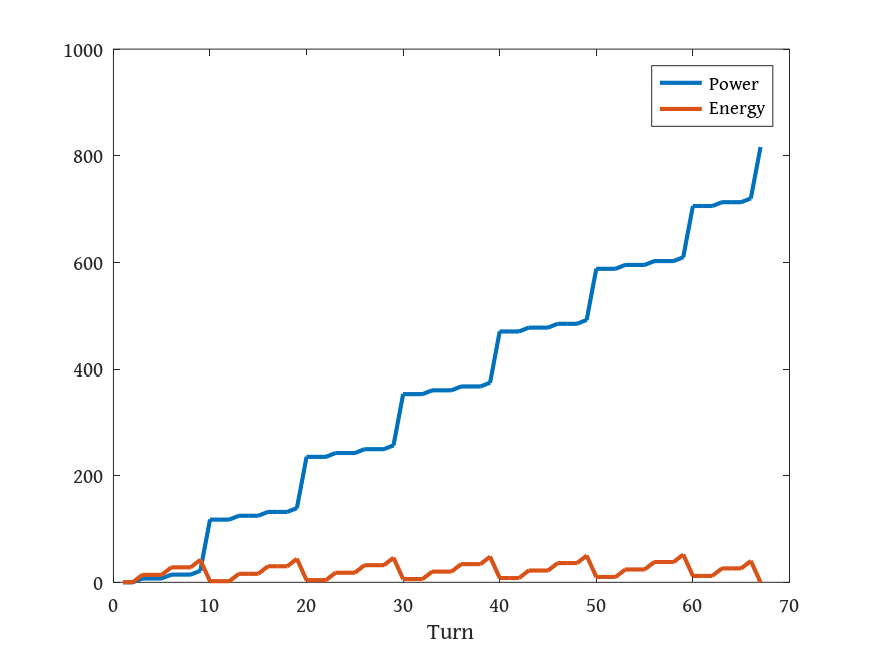
\includegraphics[width=\textwidth]{octave/greninja.png}
  \caption[Damage cycle]{Water Shuriken + Hydro Cannon (7 round cycle, 67 turns)}
\end{figure}

If we expand over multiple cycles of Fast and Charged Attack, we can
 generalize to situations with excess Energy. We know $E_{Charged} \times
 E_{Fast}$ will be a multiple of both the generated and consumed Energy, so
 simply consider $E_{Charged}$ cycles, each of which throws an average of
 $\frac{E_{Charged}}{E_{Fast}}$ Fast Attacks followed by one Charged Attack.

\[ P_{cycles} = E_{Charged} \times (\frac{E_{Charged}}{E_{Fast}} \times P_{Fast} + P_{Charged}) \]

 The number of Fast Attacks in a cycle is actually always either
 $\lfloor\frac{E_{Charged}}{E_{Fast}}\rfloor$
 or $\lceil\frac{E_{Charged}}{E_{Fast}}\rceil$ (iff $E_{Charged}$ is a multiple of
 $E_{Fast}$, these two expressions are equal, and the number of Fast Attacks
 per Charged Attack is constant). Normalize for the total time:

\[ F_{cycles} = \frac{P_{cycles}}{E_{Charged} \times (\frac{E_{Charged}}{E_{Fast}} \times T_{Fast} + T_{Charged})} \]

This has only exacerbated one of the problems we mentioned before: we may
  not get to throw all these Attacks!
Suppose we have some constant chance $0 < L_{KO} \leq 1$ of being knocked out or
 substituted following each Attack we launch, the probability of being
 in to throw the $N$th Attack is $(1 - L_{KO})^{N-1}$.
We could thus define an expected damage from Attack $N$:

\[ E_D(N) = \overline{P} \times (1 - L_{KO})^{N-1} \]

and a cumulative expected damage through $N$ Attacks:

\[ E_{TD}(N) = \sum^N_{i=1} \overline{P} \times (1 - L_{KO})^{i-1} \]

This is a geometric series where $a = \overline{P}$ and $r = 1 - L_{KO}$.
Since $0 \leq r < 1$, this series converges to

\[ E_{TD}(\infty) = \sum^\infty_{i=1} \overline{P} \times r^{i-1} = \frac{\overline{P}}{1 - L_{KO}} \]

Of course, our chance of being knocked out is usually not constant across
 Attacks, but rather an immediate function of our remaining HP and any
 damage we are about to absorb.

\section{Breakpoints}
\label{sec:breakpoints}
\textbf{FIXME}

\section{3x3 battles}
\label{sec:3x3}
Two teams of three Pokémon each are locked in mortal combat.
Each team has one champion fighting at any given time.
The team is ordered: the first Pokémon will lead, and should that Pokémon
  faint, the second Pokémon will come in unless the Trainer specifies otherwise.
An active Pokémon can be substituted, but the Trainer cannot perform another
  such substitution for fifty seconds.
Each Trainer has two shields, and will be given the option to use one each time
  the opponent uses a charged attack (assuming one is left).
The decision must be made before the attack is identified.
There is a four minute (240 second) timer on Trainer Battles, which is not displayed
  until there are twenty seconds remaining or less.
If this timer expires, the Trainer with the most Pokémon remaining wins.
If they have an equal number of Pokémon, the Trainer with less damage to their
  Pokémon (by percentage) wins.

Charged attacks are purchased with energy, fast attacks with time.
Each turn can be split into two halves, a ``top half'' and ``bottom half''.
Attacks are launched and substitutions are made in the top half, and damage is accounted in the bottom half.
Once a fast attack is started, the Trainer cannot do anything until it is complete.
Launching a charged attack brings the opponent's ongoing fast attack to its conclusion.
Damage from charged attacks is inflicted before damage from fast attacks,
  but damage from fast attacks can be inflicted simultaneously.
Charged attacks cannot be simultaneous; if both Trainers launch a charged attack
  on the same turn, one goes first,and can knock out the opponent before it
  launches its attack.
The Pokémon that goes first (``Charged Move Priority'') is the one with the
  higher $Mod_A$ (recall that this is base attack plus $IV_A$).
Shadow status does not factor into consideration, nor do any active buffs.

\subsection{GO Battle League}
\label{subsec:league}
\textbf{FIXME}

\subsection{Team GO Rocket}
\label{subsec:rocket}
Pokéstops will sometimes go black, indicating takeover by a Team GO Rocket Grunt.
There are two: Female Grunt and Male Grunt.
Trainers can engage in a 3x3 battle with the Grunt (it is not necessary to battle to
  spin the Pokéstop).
The Grunt will employ three Shadow Pokémon, and will usually have a theme type.
This type is indicated by their dialogue (\autoref{table:taunts}).
\begin{table}
\centering
\begin{tabular}{lr}
Type & Taunt\\
\Midrule
  Bug & Go, my super bug Pokémon!\\
  Dark & Wherever there is light, there is also shadow.\\
  Dragon & ROAR! ...How'd that sound?\\
  Electric & Get ready to be shocked!\\
  Fairy & Check out my cute Pokémon!\\
  Fighting & This buff physique isn't just for show!\\
  Fire & Do you know how hot Pokémon fire breath can get?\\
  Flying & Battle against my Flying-type Pokémon!\\
  Ghost & Ke... ke... ke... ke... ke... ke!\\
  Grass & Don't tangle with us!\\
  Ground & You'll be defeated into the ground!\\
  Ice & You're gonna be frozen in your tracks.\\
  Normal & Normal does not mean weak.\\
  Poison & Coiled and ready to strike!\\
  Psychic & Are you scared of psychics that use unseen power?\\
  Rock & Let's rock and roll!\\
  Steel & You're no match for my iron will!\\
  Water & These waters are treacherous!\\
\end{tabular}
\caption{Team GO Rocket Grunt taunts and typings}
\label{table:taunts}
\end{table}
Other taunts indicate mixed teams.
Grunts make use of neither shields nor substitution.
Their teams are static across the course of a month.

Defeating a Grunt will award one-sixth of a Rocket Radar.
Once the Rocket Radar is assembled and equipped, the Trainer can meet Leaders.
One of Arlo, Cliff, or Sierra can take over a Pokéstop.
These battles are similar, except that Leaders will employ shields against the first two charged attacks thrown.
Their teams are randomly chosen from a small set of possibilities that changes each month
  (each Leader's first Pokémon is constant across the month; the second and third are selected
  from groups of three).
Defeating a Leader consumes your Rocket Radar.
After winning against a Grunt or Leader, you will have an encounter with their first Pokémon.
Grunts and Leaders sometimes fly around in a gaudy Team GO Rocket balloon,
  and can be fought there.

\section{Nx1 battles}
\label{sec:nx1}
One Pokémon fends off a number of simultaneously attacking Trainers,
  each of whom has one Pokémon active at a time.
There is a timer of 180 seconds for raids below the 5🟉 difficulty level,
  and a timer of 300 seconds for 5🟉 raids.
\textbf{FIXME}

\subsection{Gyms}
\label{sec:gyms}
A team occupies an open gym by leaving a defender there.
All defenders must belong to Trainers from the same team.
Up to six defenders can be left in a gym at once, but only one
  may be left per Trainer, and that Pokémon must have full health.
A Trainer cannot leave their Buddy Pokémon, nor any Mythical nor Legendary
  Pokémon (Meltan and Melmetal excepted).
The Pokémon will remain in the Gym until defeated; it cannot be recalled.
While in the Gym, the Pokémon still counts against the Trainer's storage,
  but it cannot be interacted with in any way save feeding it Berries.
Berries can be fed to any Pokémon defending a coaligned Gym, though
  each defender can consume only ten berries per thirty minutes.
While the gym is controlled by a Raid Boss, the defenders cannot be challenged,
  nor fed berries.

Pokémon defending the gym steadily lose HP (``motivation'') at a rate
  based on their CP (\autoref{sec:cp}).
\textbf{FIXME}

\subsection{Raids}
\label{sec:raids}
Mysterious eggs sometimes appear in gyms, together with countdowns.
When the countdown expires, the egg hatches, revealing a powerful Boss Pokémon.
This Pokémon will hold the gym for some amount of time (displayed as another countdown), usually 45 minutes.
During this time, up to twenty Trainers can come together to ``raid'' the gym.
Each trainer provides a team of six Pokémon.
If all six are defeated, their Trainer can optionally continue with another team of six.
Only one Pokémon of each Trainer is active at a time, but there is unlimited substitution within the team.
These raids have their own time limits, and the raid ends when the Pokémon is defeated, no more Pokémon remain fighting,
  or the timer expires.

A raid gym has zero or more associated lobbies, each capable of holding twenty Trainers.
Empty lobbies are immediately destroyed.
Upon entering a raid gym, a Trainer is placed in an existing lobby if there is space.
A new lobby is otherwise created for the Trainer, and a 120 second timer starts.
At the end of this timer, any Trainers in the lobby will begin the raid.
Different lobbies will each fight their own instance of the boss.
Taking part in a local raid requires a Raid Pass or a Premium Battle Pass,
  and a remote raid requires a Remote Raid Pass.
Showing a pass is required to enter the lobby, but the pass is only consumed when the raid starts.
Involved Trainers can reattempt a failed raid without a second pass.

Shadow raids are backed by Team GO Rocket, and feature Shadowed bosses.
Shadow bosses ranked 3🟉 or more will enter a dangerous ``enraged'' state after losing about ⅓ of their HP.
While enraged, the Pokémon enjoys higher attack and defense, regenerates HP, and is surrounded by a purple aura.
Eight purified gems will subdue an enraged boss, as will falling to about 15\% of original HP.
Each Trainer can use up to five purified gems, with a five second delay between uses
 (note that this is insufficient to subdue the boss, making 3🟉+ shadow raids
 very difficult for solo Trainers).
Transitions into the enraged and subdued states are noted with messages.

Boss Pokémon share base ATK and DEF with their normal brethren, with a 15/15/0 IV\@.
Their MHP is greatly augmented (\autoref{table:raidmhp}).
Shadow bosses sometimes get a further boost to MHP\@.
\begin{table}
\centering
\begin{tabular}{llll}
  Tier & MHP & Shadow MHP & Time (min)\\
  \Midrule
  1🟉 & 600 & 600 & 3 \\
  2🟉 & 1,800 & n/a & 3\\
  3🟉 & 3,600 & 4,000 & 3\\
  4🟉 & 9,000 & n/a & 5\\
  5🟉 & 15,000 & 15,000 & 5\\
  Elite & 20,000 & n/a & 5\\
  Primal & 22,500 & n/a & 5\\
  6🟉 & 22,500 & n/a & 5\\
\end{tabular}
\caption{MHP for raid bosses}
\label{table:raidmhp}
\end{table}
A successful raid is followed by a ``Bonus challenge'', an encounter with the Boss Pokémon.
This Pokémon will have its own IVs, and the same base stats as any other member of its species.
The encounter uses a fixed number of Premier balls, though the Trainer can also
  use a Master ball if one is available.
Berries can be used, and have the same effects as they do in normal encounters.

\subsection{Raid Achievements}
\label{subsec:raidachievements}
\textbf{FIXME}

%\begin{figure}[hb]
%  \begin{minipage}[t]{0.3\textwidth}
%    \begin{center}
%    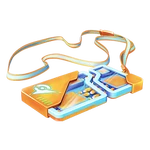
\includegraphics[width=\textwidth]{images/raidpass.png}
%    \end{center}
%    \caption*{Raid pass}
%    \label{fig:raidpass}
%  \end{minipage}
%  \begin{minipage}[t]{0.3\textwidth}
%    \begin{center}
%    
\includegraphics[width=\textwidth]{images/remoteraidpass.png}
%    \end{center}
%    \caption*{Remote raid pass}
%    \label{fig:remotepass}
%  \end{minipage}
%  \begin{minipage}[t]{0.3\textwidth}
%    \begin{center}
%    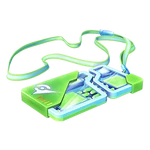
\includegraphics[width=\textwidth]{images/battlepass.png}
%    \end{center}
%    \caption*{Premium battle pass}
%    \label{fig:battlepass}
%  \end{minipage}
%\end{figure}

\subsection{Max battles}
\label{sec:maxbattles}
A Dynamax or Gigantamax Pokémon occupies a Power Stop for a period of hours to days.
A team of up to four trainers can fight a Dynamax Battle, each providing up to
  three Dynamax, Gigantamax, or Crowned Pokémon (12 total).
A Gigantamax Battle supports up to ten such teams (forty total Trainers, 120 total Pokémon).
Unlike a Raid, new Pokémon cannot be introduced to replace their fallen comrades.
Max Battles introduce a ``Max Meter'', which fills based on damage inflicted and
  energy packs recovered during the battle.
There is a distinct Max Meter for each team, when applicable.
Once it fills, active Pokémon enter their Dynamax or Gigantamax forms, and perform
  up to three Max Moves.
They will not be attacked in this form.
After all three moves, they return to their normal form, and the Max Meter returns to zero.
Trainers whose Pokémon have all fainted can cheer along their teammates,
  helping the Max Meters (all, not just their team's) fill faster.

The majority of damage is likely to be dealt while in Max form.
Filling the Max Meter is essential, as is keeping elite Max forms alive.
A basic strategy for Max battles is thus to do most attacking with a Pokémon having
  high defense and MHP, employing moves of low duration.
Single-turn fast attacks are ideal.
Each will advance the Max Meter, and flurries of fast attacks are likely to
 fill it faster than lengthy charged attacks.
While transitioning to Max form, swap in your most powerful attacker.
Swap them back out upon detransition, so that they are not exposed to damage.
This is a useful technique when battling Dynamax Pokémon; with Gigantamax Pokémon it is practically a necessity.

There is no explicit timer on Max battles, but after a few minutes the Pokémon
  will become ``desperate'' (this state change is announced).
Similarly to the ``enraged'' state of Shadow Raid bosses, their attacks and
  defense grow much more powerful.
Unlike rage, desperation cannot be alleviated with Purified Gems, so it
  is important to win quickly.
Take this into consideration before choosing Max Guard or Max Spirit over attacks.
A Max Mushroom will double the power of all damage inflicted in
  Max battles for a period of thirty minutes.
Entry to Max battles has a cost in Max Particles (\autoref{table:maxcosts}).
Non-local Trainers must also submit a Remote Raid Pass.
Power Stops provide up to 120 Max Particles when interacted with for the first time.
These can be collected each day, though subsequent interactions yield only 100.
300 Particles are made available after walking 2 km, but these do not stack---until
 they're collected, further walking has no effect.
Max Particles cannot be obtained between midnight and 0500h local time,
  and Max Battles can only be fought between 0600h and 2100h.
A Max Particle Pack provides 800 Particles.
\begin{table}
\centering
\begin{tabular}{lr}
Level & Max Particles\\
\Midrule
  1 & 250\\
  2 & 400\\
  3 & 400\\
  4+ & 800\\
\end{tabular}
\caption{Costs to enter Max battles}
\label{table:maxcosts}
\end{table}
\section{Potions and revives}
Damage to your Pokémon persists after a Raid, Max Battle, or 3x3 with Team GO Rocket ends.
Those which fainted will remain fainted until a Revive or Max Revive is applied.
While fainted, they cannot be brought into battle.
Powering up a fainted Pokémon will revive them with minimal HP (\autoref{sec:plevel}),
  while evolving one restores full HP (\autoref{sec:evolution}).
A regular Revive brings the Pokémon back with half of MHP; the Max Revive restores full HP.
If the Pokémon isn't fainted, but merely damaged, four levels of Potion
  restore various amounts of HP, never exceeding MHP\@.
Hyper Potions heal up 200 HP, sufficient to restore all but the bulkiest Pokémon to MHP.
For them, there exist Max Potions, which go all the way to MHP.
Potions cannot be applied to fainted Pokémon; they must first be revived.
Potions and Revives are level-gated, but once unlocked can be semi-randomly acquired
  from Gifts (\autoref{sec:gifts}),
  from advancing to a new Level (\autoref{table:levelitems}),
  from spinning Pokéstops (especially at Gyms, particularly when occupied by your team, and when you have a badge for the gym),
  in the three 7-day streak awards,
  by completing Routes,
  by winning Raids,
  and in the daily free package from the Store.
\begin{table}
\begin{center}
\begin{tabular}{ll}
Item & Effect \\
\Midrule
Potion & Restore 20 HP, not to exceed MHP\\
Super Potion & Restore 50 HP, not to exceed MHP\\
Hyper Potion & Restore 200 HP, not to exceed MHP\\
Max Potion & Restore to full MHP\\
Revive & Revive with half of MHP\\
Max Revive & Revive with full MHP\\
\end{tabular}
\end{center}
\caption{Potions and revives}
\label{table:potions}
\end{table}

\section{Nuzlocke rules}
Robert Munafo developed the fascinating ``Nuzlocke variant'' from Nick Franco's ``Hard Mode''
 for \textit{Pokémon Ruby}.
Capture the first six wild Pokémon you find.
You will become very close.
Seek out raids and Team GO Rocket\footnote{Munafo made no mention of Team GO Rocket, but I think they're appropriate.}.
If victorious, you may replace one of your six teammates with the captured raid boss or Shadow Pokémon.
Once Max Battles are unlocked, use the two Dynamax Pokémon from research.
They can be similarly replaced, but you must always have two (and only two) Max Pokémon, and they can be used only in Max Battles.
Nontransferable Pokémon do not count unless you elect to use them, in which case they
 must replace one of your core six.
Your score is the number of distinct raid bosses you have defeated, divided by the number of raids you have attempted.
Godspeed. Stout hearts.
